\documentclass[12pt]{article}
\usepackage[T1]{fontenc}
\usepackage[polish]{babel}
\usepackage[utf8]{inputenc}
\usepackage{graphicx}
\usepackage{amsmath}

\graphicspath{ {./images} }

\begin{document}

\title{{\Large}Zadanie numeryczne 9}
\date{}
\author{Jakub Heczko}

\maketitle

\section{Wprowadzenie do problemu: }
Problemem w tym zadaniu była macierz, miała ona bardzo duzo wartości, które były do siebie bardzo mało różniące się(np $\lambda$ = 1.99999999 i potem jakas inna $\lambda$ = 2). Na wykładzie i ćwiczeniach, było powiedzanie, że tego typu widmo macierzy sprawi, że metody potęgowe będą bardzo wolno zbieżne, jeśli w ogóle będzie zbieżna(potencjalna stagnacja).
\section{Uwagi: }
Postarałem się poprawić, wszystkie uwagi zawarte przez Pana Profesora w mailu, chociaż nie za bardzo rozumiałem wszystkie, na przykład jak inaczej inicjalizować te wektory macierzy, tak samo warunek stopu ten nowy z ćwiczeń, nie chce działać, chociaż jest on zaimplementowany w metodzie potegowa-odwrotna2, ja dalej bedę używać tej pierwotnej, ale użyję tego starego warunku stopu, chociaż z większą precyzją. Istotnie dobieram, również unormowany wektor losowy $v_{k-1}$, wiec prędkość zbiegu, może trochę się różnić, przy każdym uruchomieniu. Układ który, rozwiązałem to była macierz rozmiaru 4x4, nie wiem dlaczego, ale nie mogłem osiągnać dla większych wymiarów macierzy rozwiązań, które byłyby nawet choć troche zbliżone do prawdziwych, więc musze ucieć sie do takiego rozwiązania, bardzo przepraszam.
\section{Omówienie algorytmu: }
Jak wiemy, w poprzednim pdf w zadaniu 8, omówiłem metodę potęgową, pora zająć się jej bliźniakiem, czyli odwrotną metodą potęgową. Jak wiemy dowolny wektor zapisany w bazie wektorów własnych ${e_{1},e_{2},...,e_{n}}$ można zapisać jako:
\begin{center}
    \begin{math}
        \vec{v} = \sum_{i=1}^{N}\beta_{i}\vec{e_{i}}
    \end{math}
\end{center}
Również znany twierdzienie, że jeśli macierz A ma jakieś wartości własne, to jeśli obrócimy naszą macierz A, to jej wartości własne to również będą po kolei odwrotności wartości własnych naszej macierzy A. Oczywiście, aby to zachodziło nasza macierz, musi być odwracalna(det(A) != 0). Można więc zapisać w ogólności, tak jak przy naszej metodzie potęgowej, że:
\begin{center}
    \begin{math}
        A^{-1}\vec{v} = \sum_{i=1}^{N}\beta_{i}\vec{e_{i}}A^{-1} =^{(1)} \sum_{i=1}^{N}\beta_{i}\vec{e_{i}}\frac{1}{\lambda}
    \end{math}
    \end{center}
Pierwszy (1) krok wynika z tego, że nasza macierz jest mnożona razy wektor własny $\vec{e_{n}}$, więc dostaniemy naszą wartość własna. Ponieważ w metodzie potęgowej, normalnie dostalibyśmy najwiekszą na moduł wartość własną, to iż tutaj działamy na odwrotnościach to dostaniemy odwrotnośc najmniejszej wartości własnej, bo jak obrócimy najwiekszą wartość własną to stanie się ona najmniejszą wartościa naszej obróconej macierzy A, a skoro metoda potęgowa szuka największej wartości, to po kilku iteracjach wyskoczy nam wartość, która jest najmniejsza w mianowniku, czyli najwieksza, ze wszystkich odwrotności, czyli najmniejsza ze wszystkich wartości macierzy A. Standardowo, tak jak w metodzie potęgowej, należy użyć metody deflacji, aby móc szukać następnych wektorów własnych i wartości własnych, oczywiście po uwczesnym znalezeniu, pierwszej wartości, następnej drugiej wartości i tak dalej. Jest to ortogonalizacja szukanych wektorów do naszego uwcześniej znalezionego wektora.
\section{Warunek stopu: }
Użyłem najbardziej naiwnej metody stopu czyli:
\begin{center}
    \begin{math}
        ||\lambda_{n-1} - \lambda_{n}|| < \epsilon
    \end{math}
    \end{center}
Chciałem użyć tego co robiliśmy na ćwiczeniach, ale coś mi nie działa w każdym razie chodziło o wzór:
\begin{center}
    \begin{math}
        |q|\frac{|\lambda_{n}-\lambda_{n-1}|}{|q|-1} < \epsilon
    \end{math}
    \end{center}
Jest on zaimplementowany w tym samym pliku, ale w funkcji potegowa-odwrotna2.
\section{Wyniki algorytmu: }
Omówie, może najpierw co wpływa na szybkość zbiegu, nie pamiętam czy mówiliśmy to na ćwiczeniach( nic nie zapisałem w zeszycie na ten temat niestety), ale wybór wektora $v_{k-1}$ ma znaczenie, jak można zobaczyć, przy każdym nowym uruchomieniu, programu nasza zbieżność jest inna. Do tego zbieżnośc tak jak mówiłem zależy od tego czy w widmie naszej macierzy, nie mamy zbliżonych do siebie wartości. Ogólnie dla tej macierzy będziemy mieli bardzo wolną zbieżnośc .To teraz graficzne przedstawienie wyników:
\subsection*{Tutaj dla naszej funkcji odwrotnej potęgowej: }
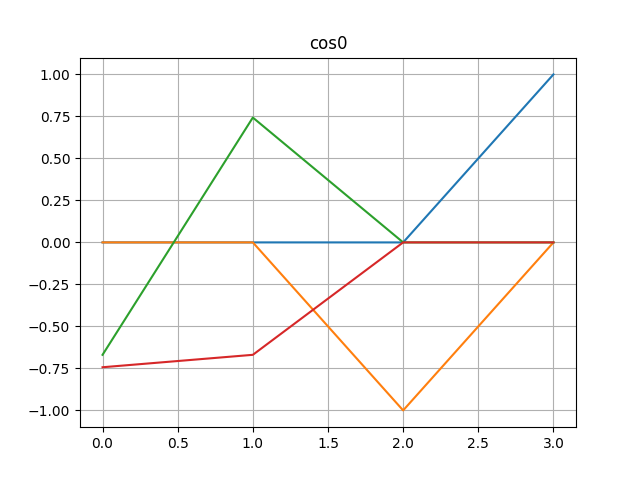
\includegraphics[width=17cm,height=8cm, keepaspectratio]{Wykres_cos0.png}
\subsection*{A tutaj dla numpy w celach sprawdzenia: }
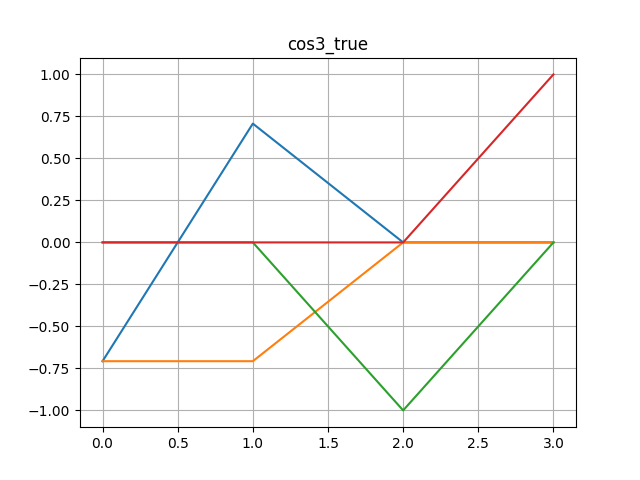
\includegraphics[width=17cm,height=8cm, keepaspectratio]{Wykres_cos3_true.png}
\newline
Widzimy, że wyniki, te tylko trochę się rozjeżdzają na początku.
\end{document}